\documentclass[journal,12pt,twocolumn]{IEEEtran}

\usepackage{setspace}
\usepackage{gensymb}

\singlespacing


\usepackage[cmex10]{amsmath}

\usepackage{amsthm}

\usepackage{mathrsfs}
\usepackage{txfonts}
\usepackage{stfloats}
\usepackage{bm}
\usepackage{cite}
\usepackage{cases}
\usepackage{subfig}

\usepackage{longtable}
\usepackage{multirow}

\usepackage{enumitem}
\usepackage{mathtools}
\usepackage{steinmetz}
\usepackage{tikz}
\usepackage{circuitikz}
\usepackage{verbatim}
\usepackage{tfrupee}
\usepackage[breaklinks=true]{hyperref}
\usepackage{graphicx}
\usepackage{tkz-euclide}
\usepackage{float}

\usetikzlibrary{calc,math}
\usepackage{listings}
\usepackage{color} %%
\usepackage{array} %%
\usepackage{longtable} %%
\usepackage{calc} %%
\usepackage{multirow} %%
\usepackage{hhline} %%
\usepackage{ifthen} %%
\usepackage{lscape}
\usepackage{multicol}
\usepackage{chngcntr}

\DeclareMathOperator*{\Res}{Res}

\renewcommand\thesection{\arabic{section}}
\renewcommand\thesubsection{\thesection.\arabic{subsection}}
\renewcommand\thesubsubsection{\thesubsection.\arabic{subsubsection}}

\renewcommand\thesectiondis{\arabic{section}}
\renewcommand\thesubsectiondis{\thesectiondis.\arabic{subsection}}
\renewcommand\thesubsubsectiondis{\thesubsectiondis.\arabic{subsubsection}}


\hyphenation{op-tical net-works semi-conduc-tor}
\def\inputGnumericTable{} %%

\lstset{
%language=C,
frame=single,
breaklines=true,
columns=fullflexible
}
\begin{document}


\newtheorem{theorem}{Theorem}[section]
\newtheorem{problem}{Problem}
\newtheorem{proposition}{Proposition}[section]
\newtheorem{lemma}{Lemma}[section]
\newtheorem{corollary}[theorem]{Corollary}
\newtheorem{example}{Example}[section]
\newtheorem{definition}[problem]{Definition}

\newcommand{\BEQA}{\begin{eqnarray}}
\newcommand{\EEQA}{\end{eqnarray}}
\newcommand{\define}{\stackrel{\triangle}{=}}
\bibliographystyle{IEEEtran}
\providecommand{\mbf}{\mathbf}
\providecommand{\pr}[1]{\ensuremath{\Pr\left(#1\right)}}
\providecommand{\qfunc}[1]{\ensuremath{Q\left(#1\right)}}
\providecommand{\sbrak}[1]{\ensuremath{{}\left[#1\right]}}
\providecommand{\lsbrak}[1]{\ensuremath{{}\left[#1\right.}}
\providecommand{\rsbrak}[1]{\ensuremath{{}\left.#1\right]}}
\providecommand{\brak}[1]{\ensuremath{\left(#1\right)}}
\providecommand{\lbrak}[1]{\ensuremath{\left(#1\right.}}
\providecommand{\rbrak}[1]{\ensuremath{\left.#1\right)}}
\providecommand{\cbrak}[1]{\ensuremath{\left\{#1\right\}}}
\providecommand{\lcbrak}[1]{\ensuremath{\left\{#1\right.}}
\providecommand{\rcbrak}[1]{\ensuremath{\left.#1\right\}}}
\theoremstyle{remark}
\newtheorem{rem}{Remark}
\newcommand{\sgn}{\mathop{\mathrm{sgn}}}
\providecommand{\abs}[1]{\left\vert#1\right\vert}
\providecommand{\res}[1]{\Res\displaylimits_{#1}}
\providecommand{\norm}[1]{\left\lVert#1\right\rVert}
%\providecommand{\norm}[1]{\lVert#1\rVert}
\providecommand{\mtx}[1]{\mathbf{#1}}
\providecommand{\mean}[1]{E\left[ #1 \right]}
\providecommand{\fourier}{\overset{\mathcal{F}}{ \rightleftharpoons}}
%\providecommand{\hilbert}{\overset{\mathcal{H}}{ \rightleftharpoons}}
\providecommand{\system}{\overset{\mathcal{H}}{ \longleftrightarrow}}
%\newcommand{\solution}[2]{\textbf{Solution:}{#1}}
\newcommand{\solution}{\noindent \textbf{Solution: }}
\newcommand{\cosec}{\,\text{cosec}\,}
\providecommand{\dec}[2]{\ensuremath{\overset{#1}{\underset{#2}{\gtrless}}}}
\newcommand{\myvec}[1]{\ensuremath{\begin{pmatrix}#1\end{pmatrix}}}
\newcommand{\mydet}[1]{\ensuremath{\begin{vmatrix}#1\end{vmatrix}}}
\numberwithin{equation}{subsection}
\makeatletter
\@addtoreset{figure}{problem}
\makeatother
\let\StandardTheFigure\thefigure
\let\vec\mathbf
\renewcommand{\thefigure}{\theproblem}
\def\putbox#1#2#3{\makebox[0in][l]{\makebox[#1][l]{}\raisebox{\baselineskip}[0in][0in]{\raisebox{#2}[0in][0in]{#3}}}}
\def\rightbox#1{\makebox[0in][r]{#1}}
\def\centbox#1{\makebox[0in]{#1}}
\def\topbox#1{\raisebox{-\baselineskip}[0in][0in]{#1}}
\def\midbox#1{\raisebox{-0.5\baselineskip}[0in][0in]{#1}}
\vspace{3cm}
\title{Assignment No.1}
\author{Abhishek Nayak}
\maketitle
\newpage
\bigskip
\renewcommand{\thefigure}{\theenumi}
\renewcommand{\thetable}{\theenumi}
Download all python codes from
\begin{lstlisting}
https://github.com/Abhishek7008/Assignment_1.git
\end{lstlisting}
%
and latex-tikz codes from
%
\begin{lstlisting}
https://github.com/Abhishek7008/Assignment_1.git
\end{lstlisting}
%
\section{Question No.1}
The sum of the digits of a two-digit number is $12$. The number obtained by interchanging the two digits exceeds the given number by $18$. Find the number ?
[CBSE/MATH/10/2006 set2- Q1(b)]
\section{Solution}
Let the tens digit of the required number be ${a_1}$ and the units digit be ${a_0}$. Then,
\begin{align}
     {a_1}+{a_0}=12\label{eq1}
\end{align}
   
Required Number is 
\begin{align}
(10{a_1}+{a_0})
\end{align}
Which can be written in vector form as
\begin{align}
    \myvec{10&1}\vec{x}
\end{align}
where 
\begin{align}
    \vec{x}=\myvec{a_1\\a_0}
\end{align}
Number obtained on reversing the digits=$(10{a_1}+{a_0})$
Therefore,
\begin{align}
  \implies (10{a_0}+{a_1})-(10{a_1}+{a_0})=18\\
   \implies{a_0}-9{a_1}=18 \\ 
  \implies{a_0}-{a_1}=2\label{eq2}
\end{align}
 Solving  \eqref{eq1}and \eqref{eq2} , can be expressed as a Matrix Equation
 \begin{align}
    \myvec{
    1 & 1 \\-1 & 1}\vec{x} = \myvec{12\\2}
 \end{align}
 \\
The augmented matrix for the above equation
is row reduced as follows:
\begin{align}
\myvec{1&1&12\\-1&1&2}\xleftrightarrow{R_2\leftarrow R_2+ R_1} \myvec{1&1&12\\0&2&14}
\\
\xleftrightarrow{R_2\leftarrow \frac{1}{2}R_2} \myvec{1&1&12 \\ 0&1&7}
\\
\xleftrightarrow{R_1 \leftarrow R_1-R_2}
\myvec{1&0&5\\0&1&7}
\end{align}

 \begin{align}
 \implies{a_1}=5 \\
\implies{a_0}=7
 \end{align}  

 As Required Number 
    \begin{align}
        &=10{a_1}+{a_0}\\
        &=10(5)+7\\
        &=57
    \end{align}
  Hence, the required number is $57$.
  \numberwithin{figure}{section}
\begin{figure}[H]
    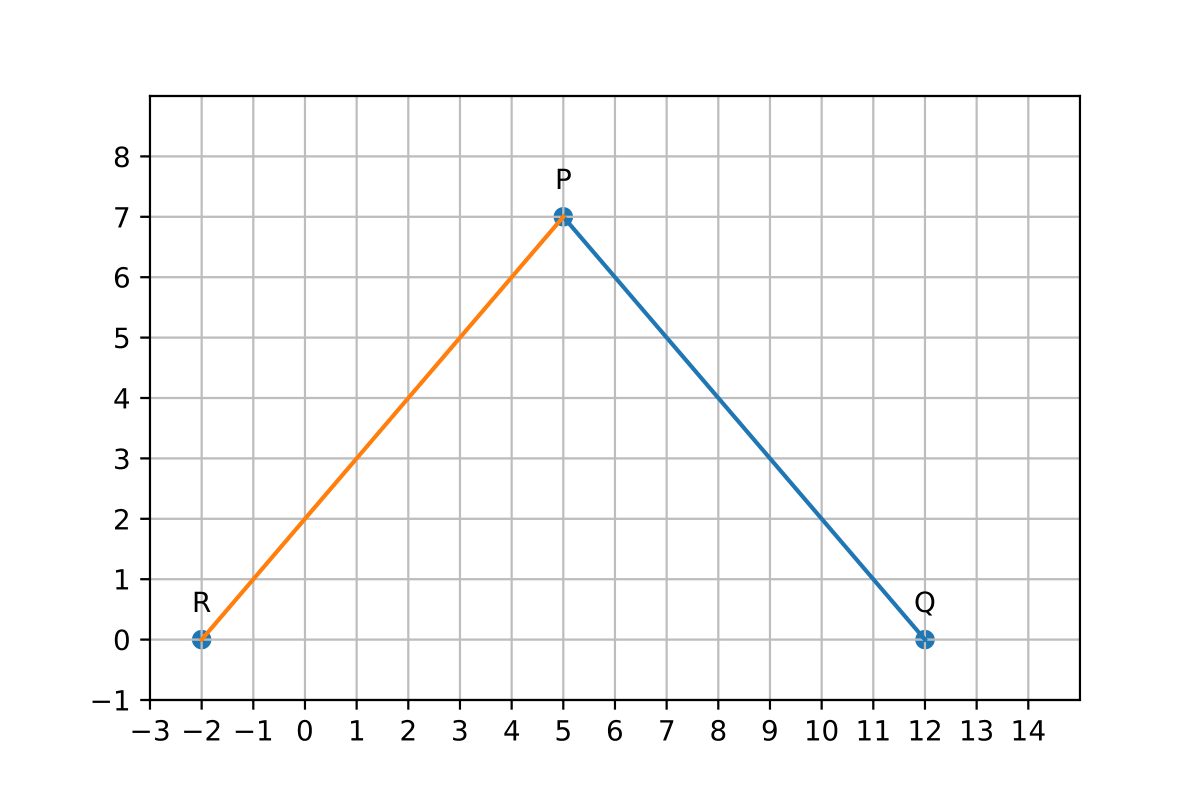
\includegraphics[width= \columnwidth]{Figure.png}
    \caption{Graphical solution}
    \label{Fig:Graphical Solution}
\end{figure}
$\therefore$ This figure verifies that two lines are intersecting at one point.
\end{document}